% PROTOKOLL Action Item
\documentclass[
   draft=false
  ,paper=a4
  ,twoside=false
  ,fontsize=11pt
  ,headsepline
  ,DIV=11
  ,parskip=full+
  ,titlepage
]{scrartcl} % copied from Thesis Template from HAW

\usepackage[ngerman,english]{babel}

\usepackage[T1]{fontenc}
\usepackage[utf8]{inputenc}

\usepackage[
    left  =4em
   ,right =4em
   ,top   =5em
   ,bottom=5em
]{geometry}

\usepackage{longtable}
\usepackage[german,refpage]{nomencl}

\usepackage{float}
%\usepackage{enumitem}
\usepackage{paralist} %compactitem
\usepackage{graphicx}
%\usepackage{url}



\usepackage{hyperref} % for a better experience

\hypersetup{
   colorlinks=true % if false - links get colored frames
  ,linkcolor=black % color of tex intern links
  ,urlcolor=blue   % color of url links
  ,citecolor=black
}

\usepackage{amsmath}

\usepackage{array}   % for \newcolumntype macro
\newcolumntype{L}{>{$}l<{$}} % math-mode version of "l" column type
\newcolumntype{R}{>{$}r<{$}} % math-mode version of "r" column type
\newcolumntype{C}{>{$}c<{$}} % math-mode version of "c" column type

\usepackage{color}
\definecolor{black}{rgb}{0,0,0}
\definecolor{darkgray}{rgb}{0.2,0.2,0.2}
\definecolor{lightgray}{rgb}{0.9,0.9,0.9}
\definecolor{blue}{rgb}{0.0,0.0,0.9}
\definecolor{orange}{rgb}{0.7,0.3,0.0}
\definecolor{green}{rgb}{0.0,0.7,0.0}
\definecolor{red}{rgb}{0.9,0.0,0.0}

\usepackage{listings, lstautogobble}
\lstset{%
   language=bash
  ,frame=single
  ,numbers=left
  ,numberstyle=\tiny\color{darkgray}
  ,stepnumber=1
  ,numbersep=5pt
  ,backgroundcolor=\color{lightgray}
  ,showspaces=false
  ,keepspaces=true
  ,autogobble=true 
  ,breaklines=true
  ,tabsize=2
  , 
  ,basicstyle=\footnotesize\ttfamily\color{black}
  ,identifierstyle=\color{black}
  ,keywordstyle=[1]\color{blue}\textbf
  ,keywordstyle=[2]\color{red}\textbf
  ,stringstyle=\color{green}
  ,commentstyle=\color{darkgray}\textit
}
  
\usepackage{caption}
\usepackage{colortbl}
\definecolor{tabgrey}{rgb}{0.85,0.85,0.85}
%using minted because of the hashtag in bash

\sloppy
\clubpenalty=10000
\widowpenalty=10000
\displaywidowpenalty=10000


\usepackage{filecontents}

\usepackage{natbib}



% set font 
%\renewcommand{\familydefault}{\sfdefault}
\usepackage{times}

\begin{document}

\selectlanguage{ngerman}
% ----------------------------------------------------------------------------
% ---------------------------------------------------------- HIER WAS MACHEN -
% -------------------------------- Metadaten wie namen und Gruppentreffen etc-
\title{Aufgabenblatt 6: Schnelles Sortieren}
\subtitle{Praktikum: Algorithmen und Datenstrukturen für technische Informatiker}
\author{Martin Witte}
\author{%
        Martin Witte 
        \\ Karl-Fabian Witte
       }
\date{\today}

\publishers{%
	\normalfont\normalsize%
	\parbox{0.8\linewidth}{\centering
	  Der Algorithmus Quicksort wird für eine spezielle Keyverteilung
	  optimiert. Die Optimierung wird erklärt. Eine empirische Messung
	  wird quantitativ aufbereitet und das Ergebnis dargeboten.
	}
}

\maketitle
\setcounter{page}{1}
\tableofcontents
\flushleft

\section{Ausgangslage}
Quicksorts Aymptotische Komplexität liegt bei $O(n)=n\log(n)$ im \texttt{best}
und im \texttt{average case}. Im \texttt{worst case} ist die Komplexität bei 
$O(n)=n^2$. Dieser Fall liegt vor, wenn als Pivotelement immer ein Extrema
der zu sortierenden Liste ausgewählt wird und somit die Rekursionstiefe
wächst. 
Für kleine Listen ist Quicksort durch das \textbf{Teile und Herrsche Prinzip}
nicht geeignet, da es mehr konstanten Aufwand kostet, 
kleinere Listen zu unterteilen
und das Pivotelement mit höherer Wahrscheinlichkeit ein Extrema ist, sodass 
der \texttt{worst case} hier öfters eintreten kann. 
Zudem summieren sich die Konstanten Operationen (Pivotsuche und Swaping des
Pivots) auf, und bei einer Listengröße von $1$ ist dies ein Aufwand, der
keinen Nutzen hat.  

\section{Problemgrößen und Schlüsselverteilung}
Es soll eine Verbesserung des Quicksortalgorithmus gefunden werde, der die 
Anzahl der Operationen verkleinert. 

Die Elemente in den Listen, besitzen einen Schlüssel $k$, der 
aufsteigend sortiert wird. In Abhängigkeit der Anzahl der Elemente $N$, 
sind die Schlüssel wie folgt zu wählen:
\[
700N \leq k \leq 800N
\] 
Zudem sind die Schlüssel in diesem Wertebereich zufällig sortiert und es
können auch doppelte Schlüssel vorkommen. Es soll aber davon ausgegangen
werden, dass die Schlüssel einigermaßen gleichverteilt sind.
Die Listengrößen 
\[
N = 10^i, i=1,2,\cdots,6
\]
werden hier untersucht.

\section{Verbesserungskonzept}
Es werden mehrere Verbesseungskonzepte implementiert.
\subsection{Quicksort mit Insertionsort für kleine Teillisten}
Um das unnötige Aufteilen von kleineren Listen zu verhindern, 
wird ab einer gewissen Mindestgröße der rekursive
Algorithmus (\textbf{Teile}) abgebrochen und durch einen anderen
Sortieralgorithmus, hier Insertionsort, ersetzt. \citep{AD}

Obwohl Insertionsort eine Komplexität von $O(n)=n^2$ hat, ist der Aufwand für 
kleine Problemgrößen $N$ meist geringer, 
da der konstante Faktor von Operationen im Quicksortverfahren hier entfällt. 

Die perfekte Abbruckgröße $S$ für die Quicksortrekursion ist nicht leicht zu
bestimmen, da diese von der Problemgröße und von der Sortiertheit der Liste 
anhängt. Es wurde daher keine mathematische Formel für die Berechnung dieser
gefunden, sodass mehrere Abbruchgrößen ($S = 10, 20, \cdots 50$) 
für die Messung verwendet werden. 

\subsection{Ausnutzung der Keyverteilung}
Ziel ist es, eine Komplexität von $O(N)$ zu erhalten.
Die Informationen über die Schlüsselverteilung wird hier verwendet, um einen
möglichst effektiven, jedoch speicherintensiven Algorithmus zu entwerfen.

Der Schlüssel wird als Index für eine extra angelegtes Array eingesetzt 
\citep{AD}. Dafür wird der Offset des Wertebereiches subtrahiert. 

\[
arrIdx = key - N*700;
\]
Es wird hierfür ein Array anlegen, welches auch entsprechend viel Platz 
zur Verfügung stellt. Dies ist nach der Schlüsseleigenschaft.
\[
700N \leq k \leq 800N \to arrSize = (801 - 700)*N
\]
($801$ da sowohl $800N$ als auch $700N$ mit eingeschlossen sind)

Da davon ausgegangen wird, dass trotz Gleichverteilung
doppelte Schlüssel existieren, wurde das Array um den Faktor 2 erweitert, um
im Fall, dass ein Schlüssel vorkommt, dieser auf das nächsten Arrayplatz
rutscht. Somit folgt:
\[
arrSize = 101*N*2, arrIdx = o.key - 700*N , arr[arrIdx] = o;
\] 
wobei $o$ ein Objekt der zu sortierenden Liste ist. 

Das Ergebnis ist eine fragmentierte Liste. Um die Lücken zu eleminieren,
wird die zu sortierende Liste mit den richtigen Werten überschrieben.
Es wird durch das Hilfsarray $arr$ durchiteriert und falls ein Plaz 
belegt ist, wird dieses Element in die Liste übertragen. 

Der Pseudocode sieht wie folgt aus:
\begin{lstlisting}
sort (list)
{
  N = list.length;
  arrLen = 2*101*N
  obj[] arr = obj[arrLen];
  
  for (i = 0; i < N; i++)
  {
    idx = (list[i].key - 700*N)*2;
    if (arr[idx] not empty ) idx++; 
    arr[idx] = list[i];
  }
  
  pos = 0;
  for (i = 0; pos < N; i++ )
  {
    if ( arr[i] not empty ){
    list[pos] = arr[i];
    pos++;
  }
}

\end{lstlisting}
Die erste Schleife iteriert $N$ mal, die zweite iteriert im 
\texttt{worst case} $arrSize = 101*N*2$. Somit erhalten wir eine 
Laufzeit von $T(N) = 203*N = O(N)$.
Im weiteren Verlauf wird dieser Algorithmus Keysort genannt.

\section{Messung}

Es werden für die Messung folgende Größen betrachtet:
\begin{itemize}
  \item[moves] Bewegungsoperationen (Speicher wird neu belegt)
  \item[compares] Vergleichsoperationen (Vergleiche von Schlüsseln)
  \item[time] Die Zeit der Sortierung (Hardware abhängig)
\end{itemize}


Die Listen werden zufällig gefüllt. Das Quicksortverfahren sucht sich 
das Pivotelement zufällig aus der Teilliste. 
Um auswertbare Werte zu erhalten, werden alle Messungen $20$ mal wiederholt
und der Mittelwert gebildet. 
Als Abbruchsgröße für die Rekursion wird eine Listengröße von $N < S_i$ 
verwendet, wobei: 
\[
S_i= 5,10,15,20,25
\]
ist.

Die Ergebnisse werden in doppellogarithmischen Diagrammen qualitativ und 
zudem in Tabellen quantitativ bewertbar dargestellt.

\begin{figure}[htp]
  \centering
  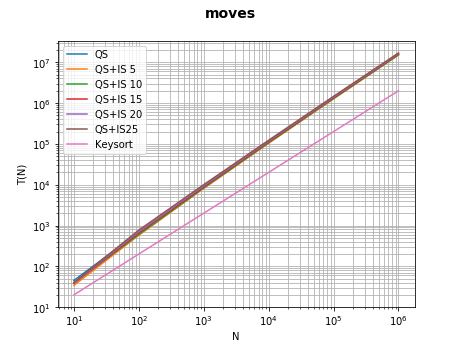
\includegraphics[width=\textwidth]{../moves.png}
  \caption[Bewegungen]{Darstellung der Anzahl der Zuweisungen der Listenenlemente $T(N)$ gegen die Problemgröße $N$}
  \label{fig:moves}
\end{figure}


\begin{table}[htp]
  \centering
  \caption[Bewegungen]{Die Anzahl der Zuweisungsbewegungen in Abhängigkeit 
  zur Listengröße $N$ der Implementationen  der Implementationen Quicksort (QS),
  Qicksort mit Isertionsort ab $S$ (QS+IS $S$) und dem Keysort}
  \label{tab:moves}
  \begin{tabular}{|r|r|r|r|r|r|r|r|}
  \hline
  $N$ & QS & QS+IS 5 & QS+IS 10 & QS+IS 15 & QS+IS 20 & QS+IS 25 & Keysort \\
  \hline
  10 & 45 & 34 & 39 & 38 & 39 & 40 & 20 \\
100 & 684 & 577 & 603 & 652 & 704 & 770 & 200 \\
1000 & 9125 & 8091 & 8322 & 8768 & 9337 & 10013 & 2000 \\
10000 & 114742 & 103880 & 106316 & 110912 & 116453 & 122629 & 20000 \\
100000 & 1378250 & 1269636 & 1292256 & 1339679 & 1394375 & 1458038 & 200000 \\
1000000 & 16073750 & 14999379 & 15210308 & 15714075 & 16233517 & 16855441 & 2000000 \\
  \hline
  \end{tabular}
\end{table}

In Abbildung \ref{fig:moves} ist nicht direkt etwas zu erkennen, jedoch sieht
man in Tabelle \ref{tab:moves} deutlich, dass der Insertionsort eine Verbesserung um ca. 1\% erbracht hat. Dabei unterschieden sich die Verfahren mit den unterschiedlichen Rekursionsabbruchkonstanten kaum von einander.   Der Abbruch bei einer Listengröße von $S=5$ hat die wenigsten Speicherbewegungen. Der Keysort liegt aber hier deutlich am besten, da er einen Aufwand von $T(N) = 2N$ hat. 


\begin{figure}[htp]
  \centering
  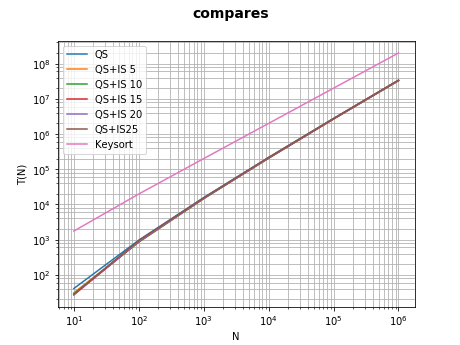
\includegraphics[width=\textwidth]{../compares.png}
  \caption[Vergleiche]{Darstellung der Anzahl der Schlüsselvergleiche 
  $T(N)$ gegen die Problemgröße $N$}
  \label{fig:compares}
\end{figure}

\begin{table}[htp]
  \centering
  \caption[Vergleiche]{Die Anzahl der Schlüsselvergleiche in Abhängigkeit 
  zur Listengröße $N$ der Implementationen Quicksort (QS),
  Qicksort mit Isertionsort ab $S$ (QS+IS $S$) und dem Keysort}
  \label{tab:compare}
  \begin{tabular}{|r|r|r|r|r|r|r|r|}
  \hline
  $N$ & QS & QS+IS 5 & QS+IS 10 & QS+IS 15 & QS+IS 20 & QS+IS 25 & Keysort \\
  \hline
  10 & 41 & 31 & 29 & 27 & 28 & 28 & 1757 \\
100 & 966 & 866 & 850 & 880 & 889 & 948 & 19821 \\
1000 & 15677 & 14592 & 14671 & 15020 & 14924 & 15352 & 200867 \\
10000 & 216537 & 209437 & 205745 & 207648 & 211078 & 216255 & 2009845 \\
100000 & 2780130 & 2687801 & 2683426 & 2682031 & 2722770 & 2752859 & 20100255 \\
1000000 & 33817025 & 33153776 & 32961227 & 32891914 & 33512717 & 33960675 & 201004834 \\
\hline
  \end{tabular}
\end{table}

Das selbe, wie in der Messung der Bewegungen, gilt auch für die Vergleiche zwischen Quicksort und der Quicksortvariante mit Insertionnsort. Abbildung \ref{fig:moves} und Tabelle \ref{tab:moves} weisen eine Verbessung von ca. 1\% auf. Der Keysort ist trotz linearer Komplexität deutlich über dem Quicksort.
Wären die Listen noch größer gewählt worden, so würde Keysort Quicksort überholen. Was aber mit einer Sehr starken Hardware erst möglich wäre.


\begin{figure}[htp]
  \centering
  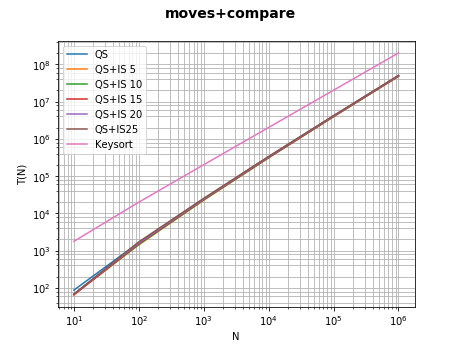
\includegraphics[width=\textwidth]{../moves+compare.png}
  \caption[Bewegungen und Vergleiche]{Darstellung der Schlüsselvergleiche und Zuweisungen zusammen $T(N)$ die Problemgröße $N$ }
  \label{fig:total}
\end{figure}


\begin{table}[htp]
  \centering
  \caption[Bewegungen und Vergleiche]{Die Anzahl der Schlüsselvergleiche und Bewegungen in Abhängigkeit 
  zur Listengröße $N$ der  der Implementationen Quicksort (QS),
  Qicksort mit Isertionsort ab $S$ (QS+IS $S$) und dem Keysort}
  \label{tab:total}
  \begin{tabular}{|r|r|r|r|r|r|r|r|}
  \hline
  $N$ & QS & QS+IS 5 & QS+IS 10 & QS+IS 15 & QS+IS 20 & QS+IS 25 & Keysort \\
  \hline
  10 & 87 & 66 & 68 & 65 & 68 & 68 & 1777 \\
100 & 1651 & 1443 & 1454 & 1533 & 1594 & 1718 & 20021 \\
1000 & 24803 & 22684 & 22994 & 23789 & 24261 & 25366 & 202867 \\
10000 & 331280 & 313318 & 312061 & 318560 & 327532 & 338885 & 2029845 \\
100000 & 4158381 & 3957438 & 3975683 & 4021711 & 4117146 & 4210898 & 20300255 \\
1000000 & 49890775 & 48153155 & 48171536 & 48605989 & 49746235 & 50816116 & 203004834 \\
\hline
  \end{tabular}
\end{table}

Die Summe aus Bewegungen und Vergleichen liegt somit im selben Verhältnis, wie man Abbildung \ref{fig:total} und \ref{tab:total} vernehmen kann. 
Gerade bei Keysort überwieden deutlich die Vergleiche.


\begin{figure}[htp]
  \centering
  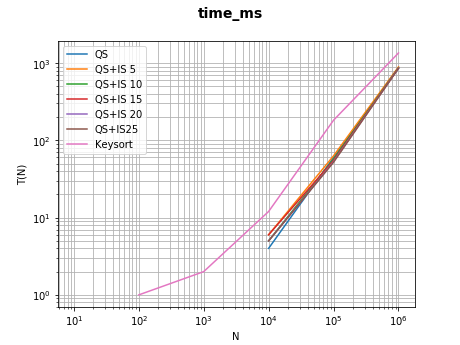
\includegraphics[width=\textwidth]{../time_ms.png}
  \caption[Zeit]{Darstellung benötigten Berechnungszeit $T(N)$ in
   Millisekunden gegen die Problemgröße $N$}
  \label{fig:time}
\end{figure}

\begin{table}[htp]
  \centering
  \caption[Bewegungen]{Die Berechnungszeit in $ms$ in Abhängigkeit 
  zur Listengröße $N$ der Implementationen Quicksort (QS),
  Qicksort mit Isertionsort ab $S$ (QS+IS $S$) und dem Keysort}
  \label{tab:time}
  \begin{tabular}{|r|r|r|r|r|r|r|r|}
  \hline
  $N$ & QS & QS+IS 5 & QS+IS 10 & QS+IS 15 & QS+IS 20 & QS+IS 25 & Keysort \\
  \hline
10 & 0 & 0 & 0 & 0 & 0 & 0 & 0 \\
100 & 0 & 0 & 0 & 0 & 0 & 0 & 1 \\
1000 & 0 & 0 & 0 & 0 & 0 & 0 & 2 \\
10000 & 4 & 6 & 5 & 6 & 5 & 5 & 12 \\
100000 & 60 & 63 & 57 & 55 & 53 & 52 & 182 \\
1000000 & 855 & 890 & 869 & 859 & 859 & 857 & 1349 \\
\hline
  \end{tabular}
\end{table}

Die Zeitmessung weißt hingegen ein auffälligeres Verhalten auf. Abbildung \ref{fig:time} und Tabelle \ref{tab:time} zeigen, dass die weniger Aufwändige Variante des Quicksorts mit Insertion sort . Da die Rekursion ständig den Stack belastet, hätte den 
reinen Quicksort mehr Zeit beansprucht, doch hier verhält sich der verbesserte
Algorithmus langsamer. Es wird vermutet, dass die Hardware bzw. die übersetzung der Virtuellen Maschine Javas die Rekursion gut optimiert.
Beim Keysort ist 200 fache Größe des Hilfsarrays ist hier der entscheidende
 limitiernede Faktor, da bei sehr großen Listen, der Zugriff auf das 
 Hilfsarray Pagefaults generiert, da dieser Bereich möglicherweise zu
 Pagefaults führt und zu systemabhängigen Laufzeiten führt.

\section{Ergebnis}

Eine Verbesserung mit dem Abbruch des rekursiven Verfahrens und der Sortierung der kleinen Teillisten mit Insertionsort ist nicht stark ausgefallen. Lediglich die Operationsanzahl hat sich um 1\% verbessert. 

Der Keysort ist nur in den Bewegungen schneller als Qicksort. Eine Verbeserung ist er somit nicht wirklich, außer es wird mit Listengrößen $N>>1M$
bearbeitet, damit die Liniarität des Aufwands den $n log n$ des Quicksorts überholt.

Eine weitere Überlegung wäre, andere Sortierverfahren auszuprobieren, wie Mergesort. 

\begin{filecontents}{doc.bib}
@book{AD
  ,author    = {Pareigis, Stephan}
  ,title     = {Algorithmen und Datenstrukturen für Technische Informatiker}
  ,year      = {2017}
  ,chater    = 2
  ,publisher = {Hochschule für Angewanste Wissenschaften Hamburg}
  ,address   = {Department für Informatik}
}
\end{filecontents}
	
	
\bibliographystyle{plainnat}
\bibliography{doc.bib}
\end{document}